% Preamble
\documentclass[11pt]{article}

% Packages
\usepackage{amsmath}
\usepackage[a4paper, margin=0.5in]{geometry}
\usepackage{graphicx} % daj an 1in jak chcesz normalniejszy margines, ale kod mi się w linii nie mieści :P
\usepackage[utf8]{inputenc}
\usepackage[T1]{fontenc}
\usepackage[polish]{babel}
\usepackage{float}
\usepackage{hyperref}
\usepackage{cleveref}
\usepackage{subfigure}

\title{Zadanie 2. Lokalne przeszukiwanie}
\author{Oskar Kiliańczyk 151863 \& Wojciech Kot 151876}
\date{}

% Document
\begin{document}

\maketitle
\newpage

\section{Opis zadania}\label{sec:opis-zadania}
Zadanie polega na implementacji lokalnego przeszukiwania w wersjach stromej (steepest) i zachłannej (greedy), z dwoma różnym rodzajami sąsiedztwa, startując albo z rozwiązań losowych, albo z rozwiązań uzyskanych za pomocą jednej z heurystyk opracowanych w ramach poprzedniego zadania.
W sumie 8 kombinacji --- wersji lokalnego przeszukiwania.
Jako punkt odniesienia należy zaimplementować algorytm losowego błądzenia, który w każdej iteracji wykonuje losowo wybrany ruch (niezależnie od jego oceny) i zwraca najlepsze znalezione w ten sposób rozwiązanie.
Algorytm ten powinien działać w takim samym czasie jak średnio najwolniejsza z wersji lokalnego przeszukiwania.
%% pytanie czy średnio najwolniejsza, czy absolutnie najwolniejsza XD

\subsection{Sąsiedztwa}\label{subsec:sasiedztwa}
W przypadku rozważanego problemu potrzebne będą dwa typy ruchów:
\begin{itemize}
\item ruchy zmieniające zbiory wierzchołków tworzące dwa cykle,
\item ruchy wewnątrztrasowe, które jedynie zmieniają kolejność wierzchołków na trasie.
\end{itemize}
Stosujemy dwa rodzaje ruchów wewnątrztrasowych (jeden albo drugi, stąd dwa rodzaje sąsiedztwa).
Jeden to wymiana dwóch wierzchołków wchodzących w skład trasy, drugi to wymiana dwóch krawędzi.
Dla ruchów wewnątrz cykli wykonujemy lokalne zamiany elementów w obrębie jednej ścieżki.

\subsection{Randomizacja kolejności przeglądania dla algorytmów zachłannych}\label{subsec:randomizacja-kolejnosci-przegladania-dla-algorytmow-zachannych}
W obu wersjach algorytmów zachłannych stosujemy randomizację wyboru.
Tworzymy listę możliwych par punktów do zamiany wewnątrz cyklu lub między dwoma cyklami.
Losowo przetasowujemy te możliwe pary, dzięki czemu kolejność przetwarzania nie jest deterministyczna.
Wybieramy pary do wymiany aż nie znajdziemy takiej, dla której zamiana daje poprawę funkcji celu.
Jeśli taka istnieje, przeprowadzamy zamianę i powtarzamy procedurę, jeśli nie ma takiej pary - kończymy przetwarzanie.

\section{Opisy algorytmów}\label{sec:opisy-alg}
\subsection{Zmiany wewnątrz cyklu}\label{subsec:zmiany-wewnatrz-cyklu}

\subsubsection{Zachłanny}


\begin{enumerate}
    \item Dla każdego z dwóch cykli startowych wykonaj następujące kroki optymalizacji:
    \begin{enumerate}
        \item Oznacz zmienną \textit{czy\_poprawiono} jako prawda.
        \item Dopóki \textit{czy\_poprawiono}:
        \begin{enumerate}
            \item Ustaw \textit{czy\_poprawiono} na fałsz.
            \item Losowo permutuj listę par indeksów miast z wyłączeniem indeksów pierwszego i ostatniego.
            \item Dla każdej pary indeksów $(i, j)$, gdzie $i < j$:
            \begin{enumerate}
                \item Oblicz zmianę długości cyklu po hipotetycznej wymianie fragmentu między $i$ a $j$.
                \item Jeśli zmiana długości jest ujemna (czyli cykl się skraca):
                \begin{enumerate}
                    \item odwróć fragment ścieżki od $i$ do $j$.
                    \item Ustaw \textit{czy\_poprawiono} na prawda i przerwij wewnętrzne pętle.
                \end{enumerate}
            \end{enumerate}
        \end{enumerate}
    \end{enumerate}
    \item item Zwróć oba zoptymalizowane cykle jako wynik działania algorytmu.
\end{enumerate}


\subsubsection{Steepest}

\begin{enumerate}
    \item Dla każdego z dwóch cykli startowych wykonaj następujące kroki optymalizacji:
    \begin{enumerate}
        \item Ustaw zmienną \textit{czy\_poprawiono} jako prawda.
        \item Dopóki \textit{czy\_poprawiono}:
        \begin{enumerate}
            \item Ustaw \textit{czy\_poprawiono} na fałsz.
            \item Zainicjalizuj zmienne \textit{najlepsza\_para} i \textit{najlepsza\_zmiana} jako zero.
            \item Dla każdej pary indeksów $(i, j)$ takich, że $i < j$, pomijając pierwszy i ostatni wierzchołek:
            \begin{enumerate}
                \item Oblicz zmianę długości cyklu po hipotetycznej zamianie fragmentu pomiędzy $i$ i $j$.
                \item Jeśli zmiana jest lepsza niż dotychczas najlepsza:
                \begin{enumerate}
                    \item Zapisz tę parę jako \textit{najlepsza\_para}.
                    \item Zapisz wartość zmiany.
                \end{enumerate}
            \end{enumerate}
            \item Jeżeli odnaleziono jakąkolwiek poprawę:
            \begin{enumerate}
                \item Odwróć fragment ścieżki między znalezioną parą.
                \item Ustaw \textit{czy\_poprawiono} na prawda.
            \end{enumerate}
        \end{enumerate}
    \end{enumerate}
    \item Zwróć oba zoptymalizowane cykle jako wynik działania algorytmu.
\end{enumerate}


\subsection{Zmiany pomiędzy cyklami}\label{subsec:zmiany-pomiedzy-cyklami}

\subsubsection{Zachłanny}


\subsubsection{Steepest}


\section{Wyniki}\label{sec:wyniki}

\subsection{Tabela wynikowa}\label{subsec:tabela-wynikowa}
\begin{table}[ht]
\centering
\resizebox{\textwidth}{!}{%
\begin{tabular}{|l|l|r|r|r|r|r|r|r|}
\hline
\textbf{Instance} & \textbf{Algorytm} & \textbf{Best} & \textbf{Avg} & \textbf{Worst} & \textbf{Avg Time} & \textbf{Best Diff} & \textbf{Avg Diff} \\
\hline
\texttt{../data/kroA200.tsp} & traverse\_greedy\_edge     & 39458  & 43643.3 & 46577  & 0.0010  & 320561 & 297093 \\
\texttt{../data/kroA200.tsp} & traverse\_greedy\_vertex   & 69190  & 80372.9 & 94789  & 0.0026  & 286837 & 258182 \\
\texttt{../data/kroA200.tsp} & traverse\_steepest\_edge   & 39408  & 43325.3 & 50129  & 0.0137  & 325160 & 297835 \\
\texttt{../data/kroA200.tsp} & traverse\_steepest\_vertex & 65888  & 79686.9 & 91978  & 0.0325  & 287177 & 259582 \\
\texttt{../data/kroA200.tsp} & traverse\_random           & 302110 & 331199  & 370208 & 0.0325  & 41606  & 9761.55 \\
\texttt{../data/kroB200.tsp} & traverse\_greedy\_edge     & 38993  & 43099.6 & 45870  & 0.0010  & 317848 & 289345 \\
\texttt{../data/kroB200.tsp} & traverse\_greedy\_vertex   & 66490  & 79094.8 & 92281  & 0.0017  & 294355 & 252270 \\
\texttt{../data/kroB200.tsp} & traverse\_steepest\_edge   & 39541  & 42884.2 & 47293  & 0.0146  & 315923 & 289159 \\
\texttt{../data/kroB200.tsp} & traverse\_steepest\_vertex & 66197  & 78607.4 & 93626  & 0.0286  & 287842 & 254715 \\
\texttt{../data/kroB200.tsp} & traverse\_random           & 293102 & 323943  & 349289 & 0.0325  & 30386  & 9234.74 \\
\hline
\end{tabular}
}
\caption{Wyniki działania algorytmów dla startu typu \texttt{randomstart}}
\label{tab:randomstart}
\end{table}


\begin{table}[ht]
\centering
\resizebox{\textwidth}{!}{%
\begin{tabular}{|l|l|r|r|r|r|r|r|r|}
\hline
\textbf{Instance} & \textbf{Algorytm} & \textbf{Best} & \textbf{Avg} & \textbf{Worst} & \textbf{Avg Time} & \textbf{Best Diff} & \textbf{Avg Diff} \\
\hline
\texttt{../data/kroA200.tsp} & traverse\_greedy\_edge     & 30293  & 32806.3 & 37011  & 0.0157  & 2503  & 291.26  \\
\texttt{../data/kroA200.tsp} & traverse\_greedy\_vertex   & 30426  & 32858.5 & 37011  & 0.0239  & 3061  & 339.52  \\
\texttt{../data/kroA200.tsp} & traverse\_steepest\_edge   & 30512  & 32486.2 & 36552  & 0.0333  & 3109  & 315.47  \\
\texttt{../data/kroA200.tsp} & traverse\_steepest\_vertex & 30595  & 32659.5 & 36552  & 0.0466  & 2503  & 222.65  \\
\texttt{../data/kroA200.tsp} & traverse\_random           & 30435  & 32934.9 & 36432  & 0.1472  & 0     & 0       \\
\texttt{../data/kroB200.tsp} & traverse\_greedy\_edge     & 30863  & 32967.3 & 36040  & 0.0166  & 3437  & 456.04  \\
\texttt{../data/kroB200.tsp} & traverse\_greedy\_vertex   & 31175  & 32955   & 36480  & 0.0229  & 2848  & 349.09  \\
\texttt{../data/kroB200.tsp} & traverse\_steepest\_edge   & 30934  & 32867.7 & 36480  & 0.0351  & 4046  & 591.07  \\
\texttt{../data/kroB200.tsp} & traverse\_steepest\_vertex & 31175  & 33043.4 & 36480  & 0.0413  & 2878  & 328.22  \\
\texttt{../data/kroB200.tsp} & traverse\_random           & 31218  & 33461.5 & 36604  & 0.1584  & 0     & 0       \\
\hline
\end{tabular}
}
\caption{Wyniki działania algorytmów dla startu typu \texttt{split\_paths\_regret\_TSP}}
\label{tab:splitpaths}
\end{table}




\subsection{Wizualizacja wyników}\label{subsec:wizualizacja-wynikow}

\subsubsection{Algorytm wymiany krawędzi (zachłanny)}
\begin{figure}[H]
    \centering
    % --- Pierwszy rząd ---
    \begin{minipage}[t]{0.45\textwidth}
        \centering
        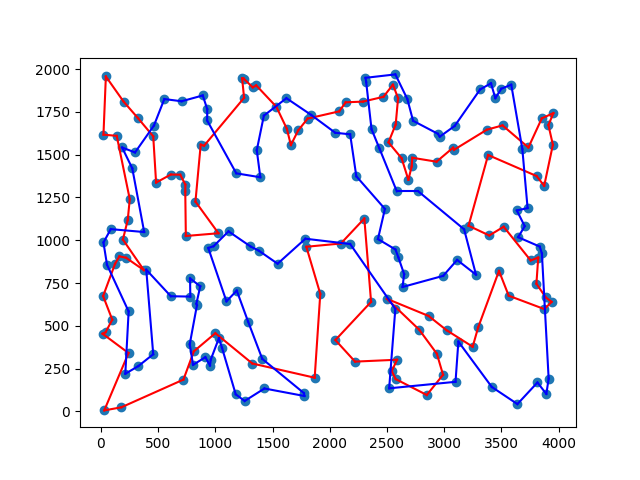
\includegraphics[width=\linewidth]{best_paths/kroA200/traverse_greedy_edge/randomstart}
        \caption{kroA200, losowy start}
    \end{minipage}
    \hfill
    \begin{minipage}[t]{0.45\textwidth}
        \centering
        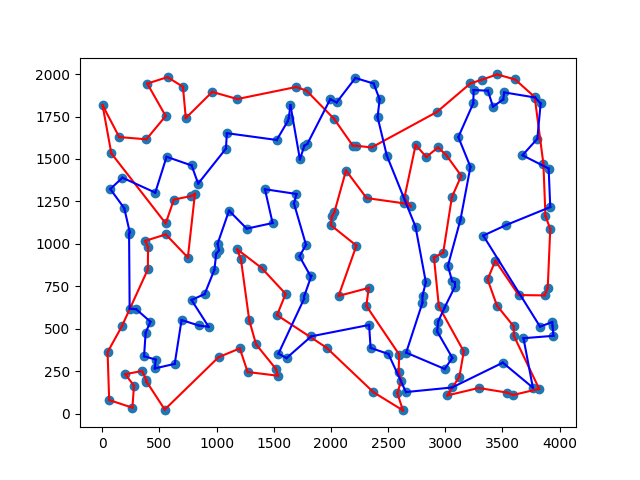
\includegraphics[width=\linewidth]{best_paths/kroB200/traverse_greedy_edge/randomstart}
        \caption{kroB200, losowy start}
    \end{minipage}

    \vspace{0.5cm}

    % --- Drugi rząd ---
    \begin{minipage}[t]{0.45\textwidth}
        \centering
        \includegraphics[width=\linewidth]{best_paths/kroA200/traverse_greedy_edge/split_paths_regret_TSP}
        \caption{kroA200, własny algorytm startowy}
    \end{minipage}
    \hfill
    \begin{minipage}[t]{0.45\textwidth}
        \centering
        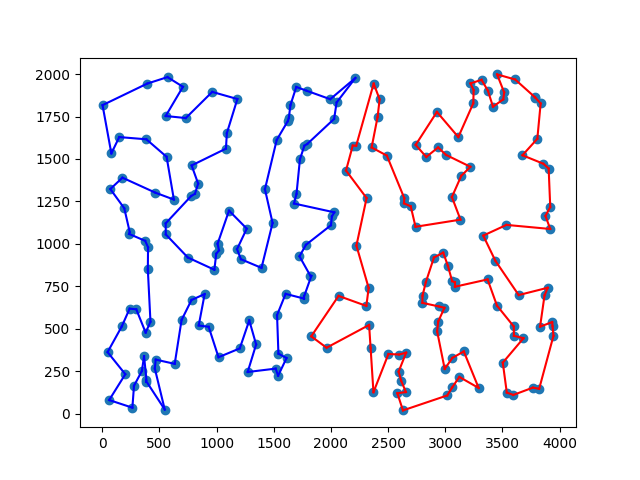
\includegraphics[width=\linewidth]{best_paths/kroB200/traverse_greedy_edge/split_paths_regret_TSP}
        \caption{kroB200, własny algorytm startowy}
    \end{minipage}
    \label{fig:minipage-greedy-edge}
\end{figure}

\subsubsection{Algorytm wymiany wierzchołków (zachłanny)}
\begin{figure}[H]
    \centering
    % --- Pierwszy rząd ---
    \begin{minipage}[t]{0.45\textwidth}
        \centering
        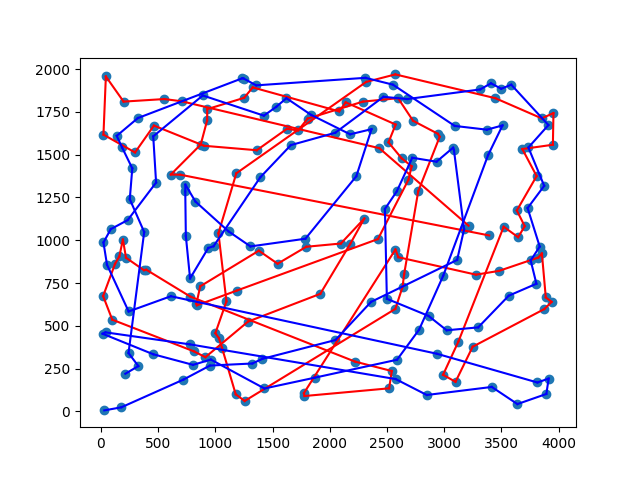
\includegraphics[width=\linewidth]{best_paths/kroA200/traverse_greedy_vertex/randomstart}
        \caption{kroA200, losowy start}
    \end{minipage}
    \hfill
    \begin{minipage}[t]{0.45\textwidth}
        \centering
        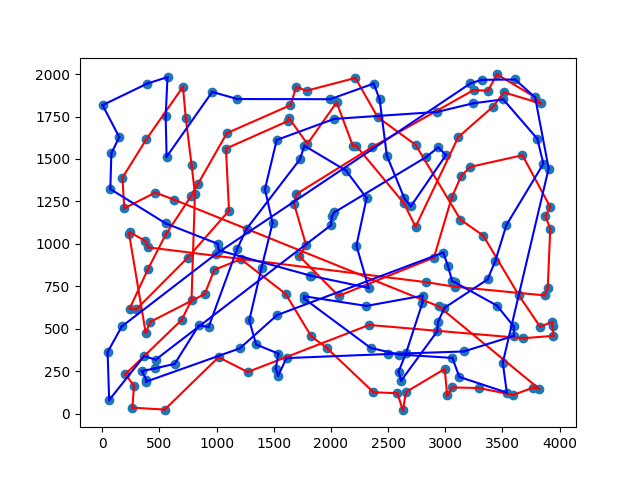
\includegraphics[width=\linewidth]{best_paths/kroB200/traverse_greedy_vertex/randomstart}
        \caption{kroB200, losowy start}
    \end{minipage}

    \vspace{0.5cm}

    % --- Drugi rząd ---
    \begin{minipage}[t]{0.45\textwidth}
        \centering
        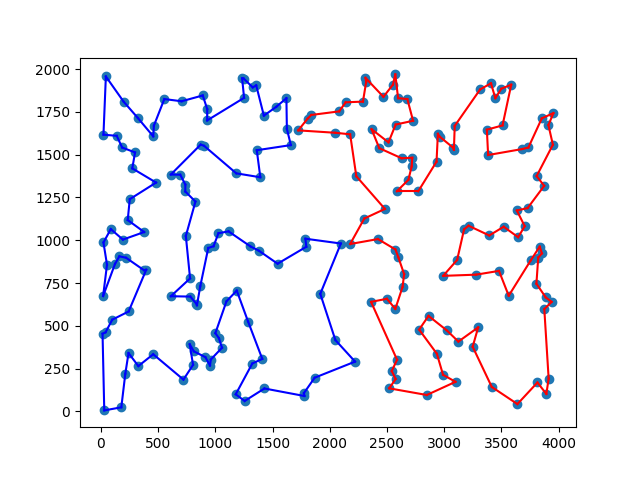
\includegraphics[width=\linewidth]{best_paths/kroA200/traverse_greedy_vertex/split_paths_regret_TSP}
        \caption{kroA200, własny algorytm startowy}
    \end{minipage}
    \hfill
    \begin{minipage}[t]{0.45\textwidth}
        \centering
        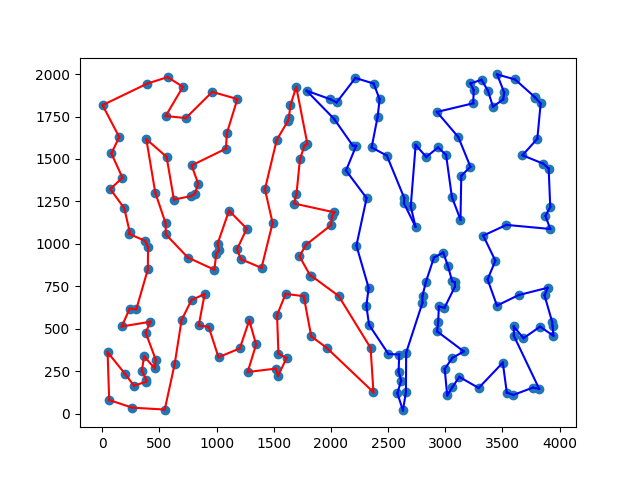
\includegraphics[width=\linewidth]{best_paths/kroB200/traverse_greedy_vertex/split_paths_regret_TSP}
        \caption{kroB200, własny algorytm startowy}
    \end{minipage}
    \label{fig:minipage-greedy-vertex}
\end{figure}

\subsubsection{Algorytm wymiany krawędzi (steepest)}
\begin{figure}[H]
    \centering
    % --- Pierwszy rząd ---
    \begin{minipage}[t]{0.45\textwidth}
        \centering
        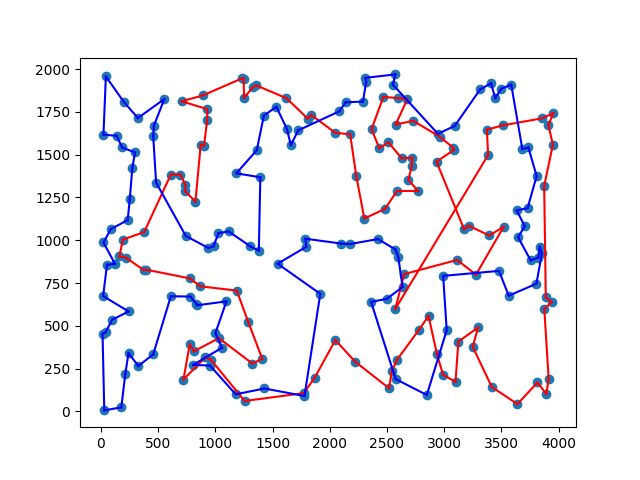
\includegraphics[width=\linewidth]{best_paths/kroA200/traverse_steepest_edge/randomstart}
        \caption{kroA200, losowy start}
    \end{minipage}
    \hfill
    \begin{minipage}[t]{0.45\textwidth}
        \centering
        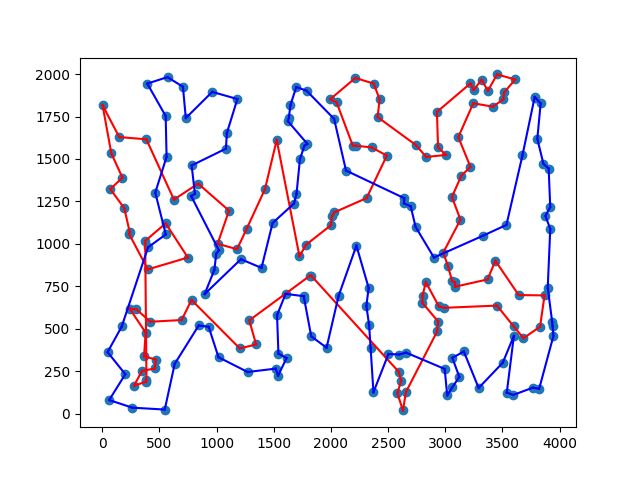
\includegraphics[width=\linewidth]{best_paths/kroB200/traverse_steepest_edge/randomstart}
        \caption{kroB200, losowy start}
    \end{minipage}

    \vspace{0.5cm}

    % --- Drugi rząd ---
    \begin{minipage}[t]{0.45\textwidth}
        \centering
        \includegraphics[width=\linewidth]{best_paths/kroA200/traverse_steepest_edge/split_paths_regret_TSP}
        \caption{kroA200, własny algorytm startowy}
    \end{minipage}
    \hfill
    \begin{minipage}[t]{0.45\textwidth}
        \centering
        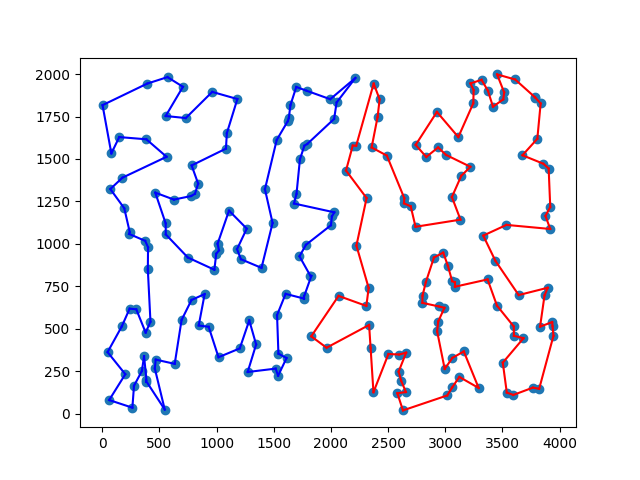
\includegraphics[width=\linewidth]{best_paths/kroB200/traverse_steepest_edge/split_paths_regret_TSP}
        \caption{kroB200, własny algorytm startowy}
    \end{minipage}
    \label{fig:minipage-steepest-edge}
\end{figure}


\subsubsection{Algorytm wymiany wierzchołków (steepest)}
\begin{figure}[H]
    \centering
    % --- Pierwszy rząd ---
    \begin{minipage}[t]{0.45\textwidth}
        \centering
        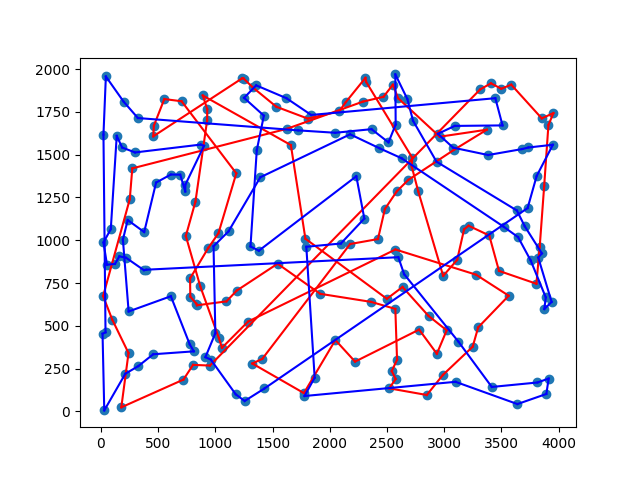
\includegraphics[width=\linewidth]{best_paths/kroA200/traverse_steepest_vertex/randomstart}
        \caption{kroA200, losowy start}
    \end{minipage}
    \hfill
    \begin{minipage}[t]{0.45\textwidth}
        \centering
        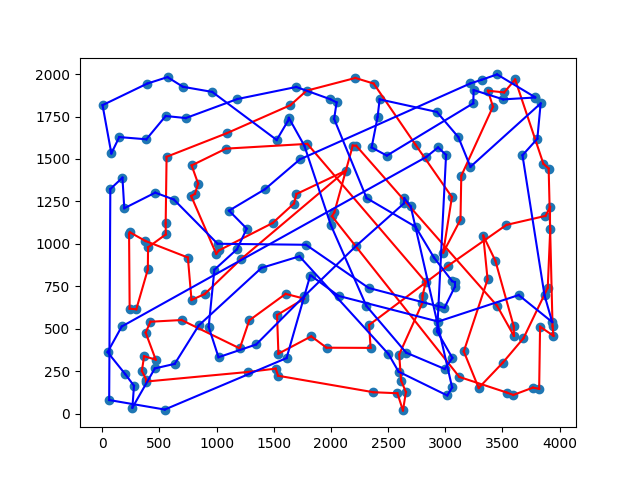
\includegraphics[width=\linewidth]{best_paths/kroB200/traverse_steepest_vertex/randomstart}
        \caption{kroB200, losowy start}
    \end{minipage}

    \vspace{0.5cm}

    % --- Drugi rząd ---
    \begin{minipage}[t]{0.45\textwidth}
        \centering
        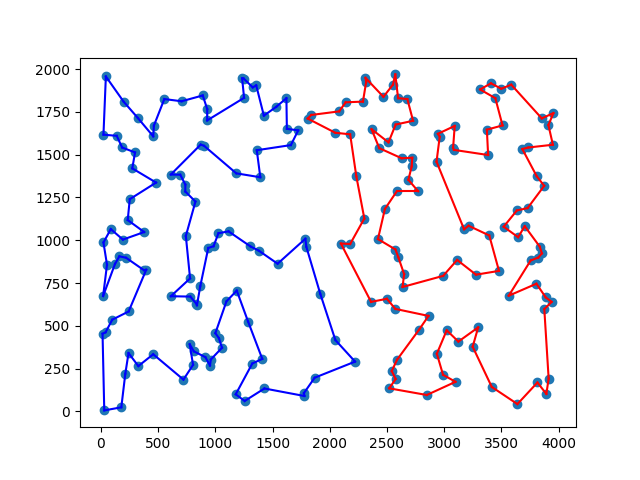
\includegraphics[width=\linewidth]{best_paths/kroA200/traverse_steepest_vertex/split_paths_regret_TSP}
        \caption{kroA200, własny algorytm startowy}
    \end{minipage}
    \hfill
    \begin{minipage}[t]{0.45\textwidth}
        \centering
        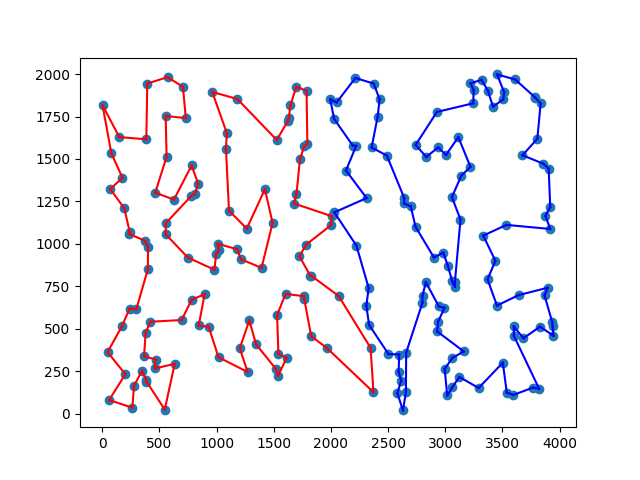
\includegraphics[width=\linewidth]{best_paths/kroB200/traverse_steepest_vertex/split_paths_regret_TSP}
        \caption{kroB200, własny algorytm startowy}
    \end{minipage}
    \label{fig:minipage-steepest-vertex}
\end{figure}


\subsubsection{Algorytm losowego błądzenia w  obu typach sąsiedztwa (random)}
\begin{figure}[H]
    \centering
    % --- Pierwszy rząd ---
    \begin{minipage}[t]{0.45\textwidth}
        \centering
        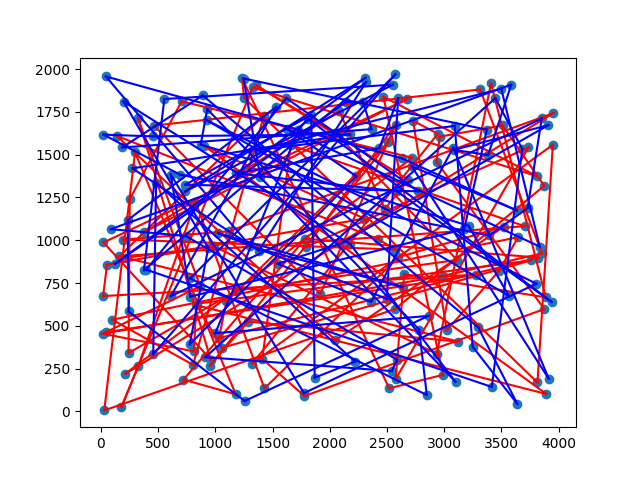
\includegraphics[width=\linewidth]{best_paths/kroA200/traverse_random/randomstart}
        \caption{kroA200, losowy start}
    \end{minipage}
    \hfill
    \begin{minipage}[t]{0.45\textwidth}
        \centering
        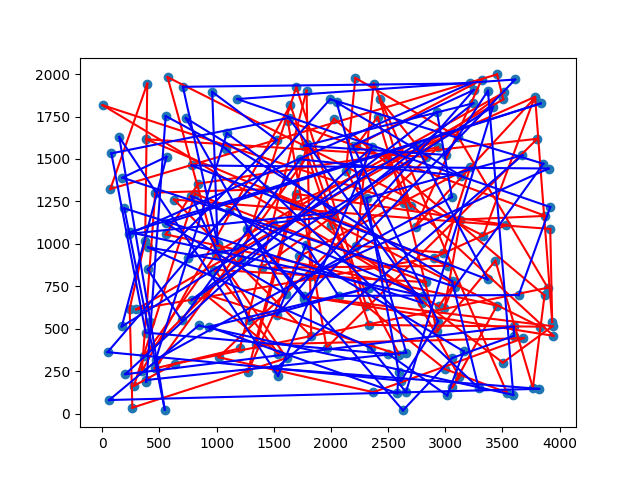
\includegraphics[width=\linewidth]{best_paths/kroB200/traverse_random/randomstart}
        \caption{kroB200, losowy start}
    \end{minipage}

    \vspace{0.5cm}

    % --- Drugi rząd ---
    \begin{minipage}[t]{0.45\textwidth}
        \centering
        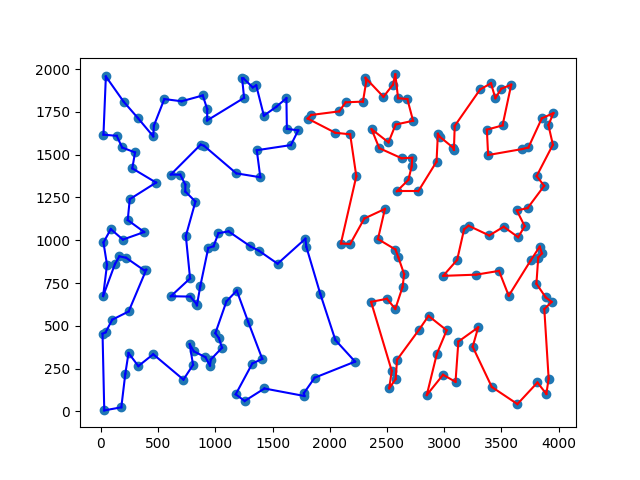
\includegraphics[width=\linewidth]{best_paths/kroA200/traverse_random/split_paths_regret_TSP}
        \caption{kroA200, własny algorytm startowy}
    \end{minipage}
    \hfill
    \begin{minipage}[t]{0.45\textwidth}
        \centering
        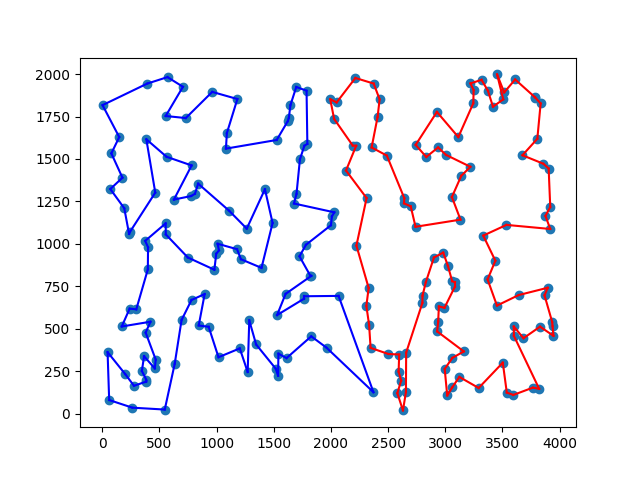
\includegraphics[width=\linewidth]{best_paths/kroB200/traverse_random/split_paths_regret_TSP}
        \caption{kroB200, własny algorytm startowy}
    \end{minipage}
    \label{fig:minipage-random}
\end{figure}

\section{Link do repozytorium}\label{sec:link-do-repo}
Kod źródłowy w repozytorium GitHub dostępny pod linkiem: \\
\href{https://github.com/KotZPolibudy/PUT_IMO/tree/main/Local_search}{Repozytorium Local Search}.

\end{document}
